\subsection{GPU Background}  \label{GPUBackground}
We provide a high-level description of the Nvidia GTX 680, depicted in Figure~\ref{Nvidia680Arch}.
We describe this particular chip because it was used in our experimental evaluation, but also because it is representative of current GPUs.
In particular, the most recent offering by Nvidia, the GTX YYYY uses the same basic Kepler architecture~\cite{????}, although the number of cores, memory/cache sizes, and some micro-architectural details will differ.

The GTX 680 consists of eight \emph{streaming multiprocessors} (SX), 
each of which contains 192 computing cores, 8,1092 registers, a 16KB L1 cache and a small, 48KB software managed on-chip memory called \emph{shared memory}, accessible to all cores of the SX.\footnote{ 
	Each SX also contains a texture cache and a constant cache, 
	but they are of no concern and hence not considered in this paper.}
A 512KB L2 cache is shared by all SXs, and the L2 cache, organized into four banks, is connected to 2GB DRAM memory called \emph{global memory}.
We refer to this global memory as \emph{GPU memory} in this paper 
to differentiate it from CPU main memory.
Access latency to registers, L1, shared memory, L2 and DRAM is 10, 80, 80, 210, and 340 cycles, respectively.
The theoretically maximum bandwidth from L1, shared memory, L2 and DRAM is 190.7GB/s, 190.7GB/s, 512GB/s, and 160GB/s, respectively.
\todo{fact check these numbers}


\begin{figure}
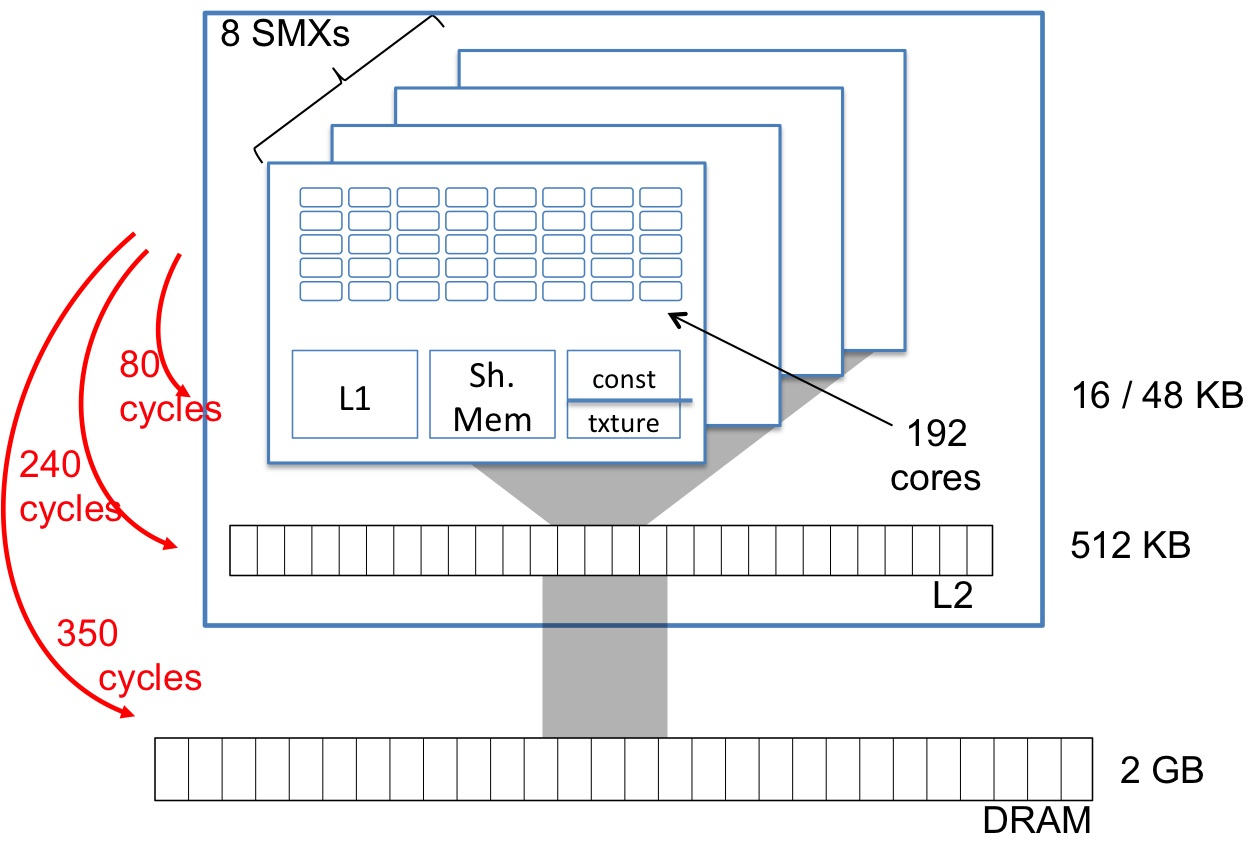
\includegraphics[width=\linewidth]{Nvidia680Arch.jpg}
\caption{Architecture of the Nvidia GTX 680}
\label{Nvidia680Arch.jpg}
\end{figure}

The GPU is connected to the CPU through a bidirectional PCIe link with 70 Gbps maximum throughput in each direction. \todo{factcheck the 70 Gbps}
The GPU has multiple DMA engines capable of
transferring data via this link between CPU memory and GPU memory. 
However, the DMA engine can only access memory CPU-side that has been pinned so that
it will not be paged out by the operating system.
The DMA engines also provide GPU cores direct (but slow) access to CPU memory.

The term \emph{kernel} is used to denote the function that executes on the 
GPU by a collection of threads in parallel.
The programmer configures the kernel to be executed by a given number of GPU threads.
These threads are grouped into {\it thread blocks} as configured by the programmer, with a maximum 2048 threads per thread block.
Each thread block is assigned to a SX by a hardware scheduler. 
Threads of a thread block are further divided into groups of 32, called \emph{warps}. 
The threads in a warp execute in lock-step 
because groups of 32 cores share the same instruction scheduler.
This lock-step execution will lead to {\it thread divergence} if,
on a conditional branch, threads within the same warp take different paths.
Thread divergence can lead to serious performance degradations. 
However, inter-warp divergence does not negatively impact performance.

\todo{Not sure what else would be important here...}

